\chapter{Specification}
\section{Satellite catching process}
\subsection{Choice of the process}

\qquad In order to catch and de-orbit a satellite in GEO, we considered the following usable tools :
\begin{itemize}
	\item Net
	\item Harpoon
	\item Claw
	\item Magnet
\end{itemize}

Other solutions such as towing the satellite or simply removing them from GEO were not considered as they either did not fit our program or would create too much strain on our spacecraft.\\

We then took a closer look at the feasibility of each solution and compared the advantages and disadvantages :
\begin{center}
	\begin{tabular}[H]{|c|c|c|c|}
		\hline
		\textbf{Solution} & \textbf{Advantages} & \textbf{Drawbacks} & \textbf{Feasibility}\\
		\hline
		\textbf{Net} & Cheap, simple, low mass &Slow, hard to handle & Yes (JAXA, ESA)\\
		\hline
		\textbf{Harpoon} & Fairly cheap & Can create more debris& Yes (ESA)\\
		\hline
		\textbf{Claw} & Safer & Mechanical, moving parts& WIP (CleanSpace One)\\
		\hline
		\textbf{Magnet} &Adjustable, no moving parts & Higher mass, needs power& Research State\\
		\hline
	\end{tabular}
\end{center}

As the main focus of our mission is reliability and re-usability, we made the choice of using magnets to catch and hold the satellite we would like to de-orbit.

\subsection{Magnetic solution}
\qquad Even though we decided that we would use magnets, we needed to make sure it was feasible and to lower the drawbacks related to this solution as much as possible. The first precision we need to make is that we will be using electromagnets in order to regulate the intensity of the current in the coil of it, thus, modulating the attraction force so the contact between our spacecraft and the satellite will not be made at high velocity, avoiding damages and space debris creation. \\

Even though it is still at the state of research, we believe that using electromagnets as our catching solution is realistic as both ESA (with ISAE SupAero) and the NASA have been considering and studying this solution since 2017.\\

However, as a matter of complexity, we will have to make assumptions in order to simplify the problem. The objective in this part is to prove that, with assumptions, this solution can be applied to our mission and to find the required energy to both catch and hold the satellite until its release.
\subsubsection{Assumptions}
In our calculations, we assumed that :
\begin{enumerate}
	\item We can consider the magnetic circuit between GREDER and the nozzle of the satellite is a closed one (no air gaps)
	\item About $0.1$\% of the satellite's mass is magnetically operable
	\item Mutual attraction is relatively low compared to the magnetic force
	\item Residuals in the alloy of the magnets' cores are neglectable
\end{enumerate}
\subsection{Sketching and Calculations}
Using the first assumption, we can use the formula for the magnetic force in a magnetic circuit with no air gap :
\begin{equation}
F = \frac{(\mu NI)^2 A}{2\mu_0 L^2}
\end{equation}
With : 
\begin{itemize}
	\item $\mu$ the magnetic permeability of the core of our magnet (determined by the alloy)
	\item $N$ the number of turns of the coil around the core
	\item $I$ the current running through the coil
	\item $A$ the cross section area of the core
	\item $\mu_0$ the magnetic constant
	\item $L$ the length of the mean magnetic circuit
\end{itemize}
In order to have a good balance between thermal properties and magnetic properties we decided to use an alloy made of $90$\% of iron and $10$\% of cobalt for our core. We decided to use this alloy as iron has the best magnetic properties (high relative magnetic permeability) and added cobalt as it has a higher Curie Temperature than iron but has a lower relative magnetic permeability.

In terms of magnet design, we chose to use a squared cross section of $5cm\times 5cm$ for the magnet core and with a length of $15cm$, made of an iron-cobalt alloy and a copper coil around it. We decided to have $135$ turns of the coil around the core with a coil diameter of $1mm$ in order to not have the wire revolutions stuck to each other. We also want to run a current of $10A$ through the coil.\\

\begin{figure}[H]
	\centering
	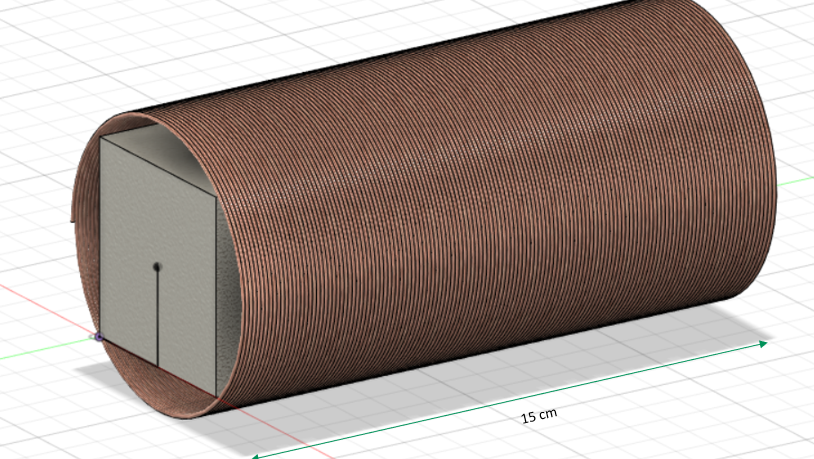
\includegraphics[width=\linewidth]{magnetCAD}
	\caption{CAD of a catching magnet}
\end{figure}


With those design choices we get the following parameters while taking into consideration that there should not be any kind of residuals in the core alloy :

\begin{itemize}
	\item $\mu_0 = 4\pi \times 10^{-7}\ H/m$
	\item $\mu = \bigg(\frac{\mu_{iron}+\mu_{cobalt}}{2}\bigg)\times\mu_0=5.868\times10^{-3}\ H/m$
	\item $N=135$ turns
	\item $I = 10\ A$
	\item $A = 25cm^2=2.5\times10^{-3}\ m^2$
	\item $\rho_{core} = \rho_{iron}\times 0.9 + \rho_{cobalt}\times0.1 = 7.9726\ g/cm^3$
	\item $\rho_{coil} = \rho_{copper} = 8.96\ g/cm^3$
\end{itemize}

We then need to find the length $L$ of the mean magnetic circuit. In order to do so, we decided to start the catching sequence at $10\ m$ from the satellite and that the target has an exploitable nozzle of $40\ cm$ of diameters which is realistic for spacecrafts in the mass range of $3\ 500\ kg$. We could then sketch the catching sequence as so (not to scale) :

\begin{figure}[H]
	\centering
	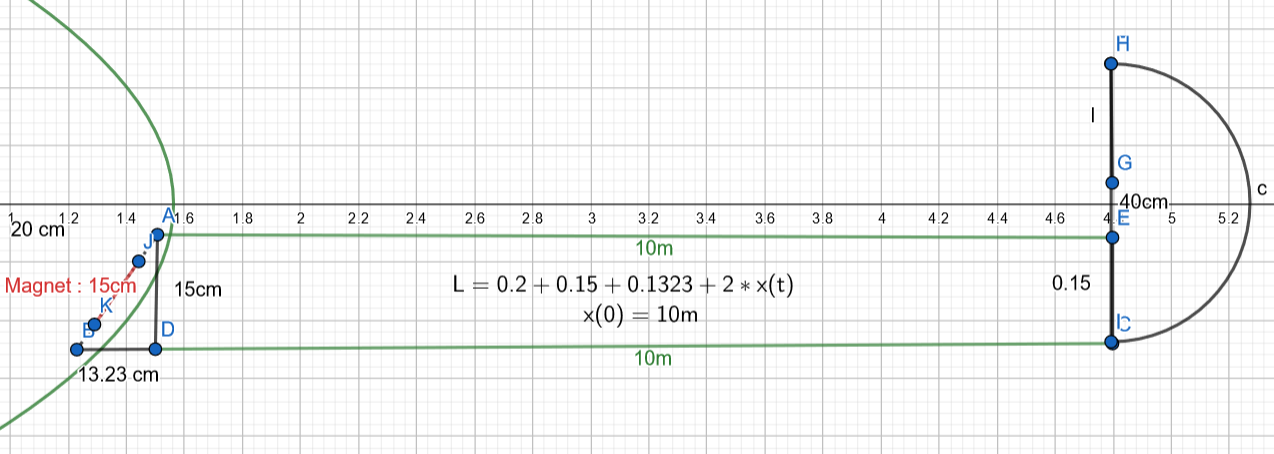
\includegraphics[width=\linewidth]{catching}
	\caption{Catching sequence (not to scale)}
\end{figure}
We can then have the length $L$ as a function of the distance between the tip of our spacecraft and the nozzle of our target. As a result we can proceed to find the feasibility of our solution with this magnet design by finding the time it would require at this state to attract the target. However, in this case, the current modulation when the target is close has not been modeled due to its complexity.\\

Considering that the force will be on one axis only and $m = 0.001\times m_{target} = 3.5\ kg$ :
\begin{align}
\vec F &= m\vec a\\
\frac{(\mu NI)^2 A}{2\mu_0 L(x)^2} &= m \times \ddot x\\
\frac{(\mu NI)^2 A}{2\mu_0 [0.2 + 0.15 + 0.1323 + 2x(t)]^2} &= m \ddot x(t)\\
\frac{(\mu NI)^2 A}{2\mu_0 [0.4823 + 2x(t)]^2} &= m \ddot x(t)
\end{align}

The catching time can then be found using $ode45$ on Matlab :
\begin{minted}[fontsize=\footnotesize, linenos, autogobble, breaklines]{matlab}
clearvars; clc;
catchtime = 1;
x0 = 10;
while 1
    [t,x] = ode45(@f3,[0:1:catchtime], [x0; 0; 0; 0]);
        if (x(catchtime ,1) >= 2 * x0)
            break
        else
            catchtime = catchtime +1;
        end
end
\end{minted}
And the function used for the $ode$ solver :
\begin{minted}[fontsize=\footnotesize, linenos, autogobble, breaklines]{matlab}
function  [Xdot] = f3(t, X)
mu = 5.686e-3; mu0 = 4 * pi * 10 ^(-7);
N = 135; I = 10; A = 0.05 ^ 2; m = 3500 ;
x = X(1); y = X(2); vx = X(3); vy = X(4);
Fmag = (mu * N * I) ^2 * A / (2 * mu0 *(2 * norm(X(1:2)) + 0.4823) ^ 2 );
Xdot = [vx; vy;  0.001 * Fmag / m; 0]; 
end
\end{minted}
We then get a catching time of $812$ seconds. As a result, we can determine the energy required to operate the magnets aswell as their masses and volumes. We are considering a holding time for approximately half an hour and we also need to verify that the magnets will be able to hold the target while we are de-orbiting.

\newpage
\section{Propellant selection}
\newpage
\section{Mass analysis}
\newpage
\hypertarget{header-n0}{%
	\section{Mass Budget - First Iteration}\label{header-n0}}

\qquad Before actually going into our mass budget, we wanted to get a reference
idea for the propellant mass so that we would be sure to be able to
achieve our \(\Delta v\). In order to get this, we decided to find a
relation between the usable propellant mass and the mass of the rest as
a ratio. This is then fixed and will also allow us to know roughly how
much propellant we need depending on the dry mass. Let \(m_{UP}\) be the
mass of usable propellant. Moreover, we would be aiming for a total initial mass of roughly $20$ to $25t$ on our last iteration. This first iteration was done with another magnet design, presented in November which consisted in two large discs of $600\ kg$ each and have then been abandoned for the second iteration.

\hypertarget{header-n3}{%
	\subsection{Coefficients \& Masses after steps}\label{header-n3}}

Considering that \(ISP = 295s\) and annotating
\(\frac{m_{UP_i}}{m_{total_i}} = K_i\) with \(i\) the burn number :

\begin{longtable}[]{@{}cccc@{}}
	\toprule
	Step & Required \(\Delta v\) in \(m/s\) & \(K_i\) & Mass after
	step\tabularnewline
	\midrule
	\endhead
	1 & 2802.4 & 0.620 & 0.38 \(m_{initial}\)\tabularnewline
	2 & 1342.2 & 0.371 & 0.239\(m_{initial}\)\tabularnewline
	3 & 522.9 & 0.165 & 0.200\(m_{initial}\)\tabularnewline
	Satellite caught & NA & NA & 0.2\(m_{initial}\) + 3500\tabularnewline
	4 & 1487.8 & 0.402 & 0.1196\(m_{initial}\) + 2093\tabularnewline
	Satellite release & NA & NA & 0.1196\(m_{initial}\) -
	1407\tabularnewline
	5 & 5.3 & 0.002 & 0.1194\(m_{initial}\) - 1404.186\tabularnewline
	6 & 72.4 & 0.0247 &\tabularnewline
	\bottomrule
\end{longtable}

\hypertarget{header-n51}{%
	\subsection{\texorpdfstring{Global equation between \(m_{UP}\) and
			\(m_{initial}\)}{Global equation between m\_\{UP\} and m\_\{initial\}}}\label{header-n51}}

\begin{longtable}[]{@{}ccc@{}}
	\toprule
	Step & \(\frac{m_{UP}}{m_{initial}}\) & Bias due to
	debris\tabularnewline
	\midrule
	\endhead
	1 & 0.620 & 0\tabularnewline
	2 & 0.141 & 0\tabularnewline
	3 & 0.039 & 0\tabularnewline
	4 & 0.0804 & 1407\tabularnewline
	5 & 0.00024 & -2.814\tabularnewline
	6 & 0.00295 & -36.68\tabularnewline
	TOTAL & 0.88359 & +1369.506\tabularnewline
	\bottomrule
\end{longtable}

We then get our general relation between the usable propellant mass and
the initial mass

\[m_{prop} = 0.88359 m_{init} + 1369.506\]

And as \(m_{initial} = m_{UP} + m_{rest}\) :

\[m_{prop} = \frac 1{0.11641}\bigg[0.88359 m_{rest} + 1369.506\bigg]\]

\(m_{rest}\) includes the dry mass and the propellant required for the
ACS.

\hypertarget{header-n90}{%
	\subsection{First iteration of mass budget}\label{header-n90}}

\hypertarget{header-n91}{%
	\subsubsection{Sub systems}\label{header-n91}}

\begin{longtable}[]{@{}cc@{}}
	\toprule
	Contributor & Mass in kg\tabularnewline
	\midrule
	\endhead
	\underline{\textbf{EPS}} & -\tabularnewline
	Fuel cells & 165.6727\tabularnewline
	H2 for fuel cell (tank included) & 10\tabularnewline
	Cables & 20\tabularnewline
	GNC & 5\tabularnewline
	Batteries & 61.3333\tabularnewline
	Actuators (for flaps) & 10\tabularnewline
	Servos & 1\tabularnewline
	\underline{\textbf{On board computer}} & 5\tabularnewline
	\underline{\textbf{Telecommunications}} & 10\tabularnewline
	\underline{\textbf{Thermal control}} & 10\tabularnewline
	\underline{\textbf{ACS/RCS}} & -\tabularnewline
	Reaction wheels & 106\tabularnewline
	ACS (without propellant) & 36.16\tabularnewline
	\underline{\textbf{\emph{Total}}} & 440.166\tabularnewline
	\bottomrule
\end{longtable}

\hypertarget{header-n120}{%
	\subsubsection{Payload}\label{header-n120}}

\begin{longtable}[]{@{}cc@{}}
	\toprule
	Contributor & Mass in kg\tabularnewline
	\midrule
	\endhead
	Magnet & 1200\tabularnewline
	\bottomrule
\end{longtable}

\hypertarget{header-n147}{%
	\subsubsection{Structure}\label{header-n147}}

\begin{longtable}[]{@{}cc@{}}
	\toprule
	Contributor & Mass in kg\tabularnewline
	\midrule
	\endhead
	Hull & 509\tabularnewline
	Wing & 54\tabularnewline
	Engine & 60\tabularnewline
	Engine frame & 51\tabularnewline
	Connectors & 25\tabularnewline
	Tanks & 350\tabularnewline
	Heat shield & 472\tabularnewline
	\underline{\textbf{\emph{Total}}} & 1521\tabularnewline
	\bottomrule
\end{longtable}

\hypertarget{header-n156}{%
	\subsubsection{Others}\label{header-n156}}

\begin{longtable}[]{@{}cc@{}}
	\toprule
	Contributor & Mass in kg\tabularnewline
	\midrule
	\endhead
	Catalyzer & 10\tabularnewline
	Lines & 25\tabularnewline
	ACS including Propellant & 672\tabularnewline
	Non usable propellant (Residuals, transient, etc.) & 200\tabularnewline
	Helium (including tank) & 30\tabularnewline
	\underline{\textbf{\emph{Total}}} & 937\tabularnewline
	\bottomrule
\end{longtable}

We then get

\[m_{rest} = m_{Sub systems} + m_{Payload} + m_{Structure} + m_{Others} = 4098.166kg\]

Which, with the previously obtained equation :

\[m_{UP} = 42\ 870.926kg\\\]

As the mixture ratio is $MR = 7.07$ and $m_{UP} = m_{UF} + m_{UOP}$\\
\begin{align*}
m_{UsableFuel} &= \frac{m_{UP}}{1 + MR} = 5\ 312kg\\
m_{UsableOxidizer} &= MR \times m_{UsableFuel} =37\ 559kg
\end{align*}

\subsubsection{Results}
We can sum this first iteration up with the following table :
\begin{center}
	\begin{tabular}[H]{|c|c|}
		\hline
		\cellcolor{gray!50}\textbf{Contributor} & \cellcolor{green!20}\textbf{Mass} (kg)\\
		\hline
		\textbf{Structure} & $1\ 521$\\
		\hline
		\textbf{Magnets} & $1\ 200$\\
		\hline
		\textbf{Sub Systems} & $440.166$\\
		\hline
		\textbf{Tank Pressurization} & $30$\\
		\hline
		\textbf{Engine} & $60$\\
		\hline
		\textbf{Catalyzer} & $10$\\
		\hline
		\textbf{Lines} & $25$\\
		\hline
		\cellcolor{gray!50}\textbf{Dry mass} & \cellcolor{green!20} $3\ 286.166$\\
		\hline
		\textbf{Non usable propellant} & $200$\\
		\hline
		\textbf{ACS/RCS Propellant} & $142. 12$\\
		\hline
		\textbf{Usable propellant} & $42\ 870.926$\\
		\cellcolor{red!50}\textbf{Total initial mass} & \cellcolor{red!50}$46\ 969.092$\\
		\hline 
	\end{tabular}
\end{center}
This first initial mass is way over what we are targeting and there are many parameters to be refined during the next iteration.
\newpage
\section{Mass Budget - Second iteration}
\qquad After refining multiple parameters and fixing others to get more accurate values, we went into the second iteration of our mass budget. Having our $I_{SP}$ changed also required another iteration in our calculation formula between the usable propellant mass the the rest of the mass.
\hypertarget{header-n422}{%
	\subsection{Coefficients \& Masses after steps}\label{header-n422}}

Considering that \(ISP = 315s\) and annotating
\(\frac{m_{UP_i}}{m_{total_i}} = K_i\) with \(i\) the burn number :

\begin{longtable}[]{@{}cccc@{}}
	\toprule
	Step & Required \(\Delta v\) in \(m/s\) & \(K_i\) & Mass after
	step\tabularnewline
	\midrule
	\endhead
	1 & 2802.4 & 0.596 & 0.404 \(m_{initial}\)\tabularnewline
	2 & 1342.2 & 0.352 & 0.261792\(m_{initial}\)\tabularnewline
	3 & 522.9 & 0.156 & 0.221\(m_{initial}\)\tabularnewline
	Satellite caught & NA & NA & 0.221\(m_{initial}\) + 3500\tabularnewline
	4 & 1487.8 & 0.382 & 0.137\(m_{initial}\) + 2163\tabularnewline
	Satellite release & NA & NA & 0.137\(m_{initial}\) -1337\tabularnewline
	5 & 5.3 & 0.0017 & 0.1368\(m_{initial}\) - 1334.73\tabularnewline
	6 & 72.4 & 0.023 &\tabularnewline
	\bottomrule
\end{longtable}

\hypertarget{header-n470}{%
	\subsection{\texorpdfstring{Global equation between \(m_{UP}\) and
			\(m_{initial}\)}{Global equation between m\_\{UP\} and m\_\{initial\}}}\label{header-n470}}
\begin{longtable}[]{@{}ccc@{}}
	\toprule
	Step & \(\frac{m_{UP}}{m_{initial}}\) & Bias due to
	debris\tabularnewline
	\midrule
	\endhead
	1 & 0.596 & 0\tabularnewline
	2 & 0.142 & 0\tabularnewline
	3 & 0.041 & 0\tabularnewline
	4 & 0.084 & 1337\tabularnewline
	5 & 0.0002 & -2.273\tabularnewline
	6 & 0.0032 & -30.699\tabularnewline
	TOTAL & 0.8664 & +1304.028\tabularnewline
	\bottomrule
\end{longtable}



This time our equation between those two masses is given by 
\begin{equation}
	m_{UsableProp} = \frac 1{0.1336}\bigg[0.8664 m_{rest} + 1304.028\bigg]
\end{equation}

\subsection{Second iteration of mass budget}

\qquad As our way of presenting our first iteration of the mass budget didn't seems clear enough to us, we decided to present it in another, more logical way :
\textbf{\underline{Structure}}
\begin{center}
	\begin{tabular}[H]{|c|c|}
		\hline
		\cellcolor{gray!50}Contributor & \cellcolor{gray!50}Mass (kg)\\
		\hline
		Hull & $192$\\
		\hline
		Tanks (including non usable propellant) & $700$\\
		\hline
		Wings & $136$\\
		\hline
		Lines & $60$\\
		\hline
		Connectors & $16$\\
		\hline
		$H_2$ tank & $12$\\
		\hline
		\cellcolor{green!30}\textbf{Structure} & \textbf{$1\ 116$}\\
		\hline
	\end{tabular}
\end{center}

\textbf{\underline{Electrical related contributors}}
\begin{center}
	\begin{tabular}[H]{|c|c|}
		\hline
		\cellcolor{gray!50}Contributor & \cellcolor{gray!50}Mass (kg)\\
		\hline
		Batteries & $241$\\
		\hline
		Fuel cells & $202$\\
		\hline
		On Board Computer & $5$\\
		\hline
		Cables & $20$\\
		\hline
		$H_2$ for fuel cells & $5$\\
		\hline
		Wing actuators & $10$\\
		\hline
		Telecommunications & $10$\\
		\hline
		GNC & $5$\\
		\hline
		Thermal Control & $10$\\
		\hline
		Magnets (Payload) & $25.65$\\
		\hline
		\cellcolor{green!30}\textbf{Electrical related contributors} & \textbf{$533.65$}\\
		\hline
	\end{tabular}
\end{center}

\textbf{\underline{ACS and RCS}}
\begin{center}
	\begin{tabular}[H]{|c|c|}
		\hline
		\cellcolor{gray!50}Contributor & \cellcolor{gray!50}Mass (kg)\\
		\hline
		Thrusters & $36$\\
		\hline
		$H_2O_2$ & $90$\\
		\hline
		Reaction wheels & $106$\\
		\hline
		\cellcolor{green!30}\textbf{ACS \& RCS} & \textbf{$232$}\\
		\hline
	\end{tabular}
\end{center}

\textbf{\underline{Propulsion}}
\begin{center}
	\begin{tabular}[H]{|c|c|}
		\hline
		\cellcolor{gray!50}Contributor & \cellcolor{gray!50}Mass (kg)\\
		\hline
		Engine & $93$\\
		\hline
		Turbopumps & $25$\\
		\hline
		Pressurization ($He$) & $1.3$\\
		\hline
		Catalyzer & $30$\\
		\hline
		\cellcolor{green!30}\textbf{Propulsion} & \textbf{$149.3$}\\
		\hline
	\end{tabular}
\end{center}

With those tables, we can deduce $m_{rest}$ :
\begin{align}
	m_{rest} &= m_{Structure} + m_{Elec} + m_{ACS\&RCS} + m_{Propulsion}\\
	m_{rest} &= 2\ 030.95kg
\end{align}
Thus,
\begin{align}
	m_{UsableProp} &= \frac 1{0.1336}\bigg[0.8664 m_{rest} + 1304.028\bigg]\\
	m_{UsableProp} &= 22\ 931kg\\
	m_{Fuel} &= \frac{m_{UsableProp}}{MR+1}\\
	m_{Fuel} &= 2841.6kg\\
	m_{Ox} &= m_{UsableProp} - m_{Fuel}\\
	m_{Ox} &= 20\ 089.89kg\\
	m_0 &= 24\ 962.41kg
\end{align}



In this second iteration with a better \(I_{sp}\) and refined values for all of the contributors, we have a large improvement as our initial mass decreased drastically.
\newpage
\section{Frozen information}
After our second iteration of the mass budget, we decided to make a list of the fixed values that we will work around in our further design.
\subsection{Frozen points}
\begin{itemize}
	\item We will do $20$ aerobrakes
	\item We will have a separate tank design
	\item $H_2O_2$ will be pressurized by its decomposition
	\item The decomposition control will be managed by rotation of the spacecraft
	\item ACS/RCS Layout similar to the Space Shuttle
	\item $H_2O_2$ catalyzers separate
	\item $H_2O_2/O_2$ separation via thermodynamic properties
	\item $H_2/O_2$ will be used in fuel cells to produce energy
\end{itemize}
\begin{center}
	\begin{tabular}[H]{|c|c|c|}
		\hline
		\cellcolor{gray!50}Data & \cellcolor{gray!50}Value & \cellcolor{gray!50}Unit\\
		\hline
		Empty raw mass & $2\ 031$ & kg\\
		\hline
		Usable propellant & $22\ 931$ &kg\\
		\hline
		\cellcolor{green!50}Total mass & \cellcolor{green!50}$24\ 962$ & \cellcolor{green!50}kg\\
		\hline
		Flowrate & $10$ & kg/s\\
		\hline
		Rocket diameter & $2$ & $m$\\
		\hline
		$I_{sp_{vacuum}}$ & $335$ & s\\
		\hline
		Thrust $F=\dot m I_{sp} g_0$ & $32 863.5$ &N\\
		\hline
		Mixture Ratio & $7.07$ & -\\
		\hline
		Wall thickness & $TBA$ & m\\
		\hline
		$H_2O_2$ internal pressure & $1.35$ & bar\\
		\hline
	\end{tabular}
\end{center}
\newpage
\section{Mass Budget - Third iteration}
As the fixed $I_{sp}$ has been refined, we went into our third iteration of the mass budget with the same process as the two previous ones.
\subsection{Coefficients \& Masses after steps}

Considering that \(ISP = 335s\) and annotating
\(\frac{m_{UP_i}}{m_{total_i}} = K_i\) with \(i\) the burn number :

\begin{longtable}[]{@{}cccc@{}}
\toprule
Step & Required \(\Delta v\) in \(m/s\) & \(K_i\) & Mass after
step\tabularnewline
\midrule
\endhead
1 & 2802.4 & 0.574 & 0.426 \(m_{initial}\)\tabularnewline
2 & 1342.2 & 0.335 & 0.283\(m_{initial}\)\tabularnewline
3 & 522.9 & 0.148 & 0.241\(m_{initial}\)\tabularnewline
Satellite caught & NA & NA & 0.221\(m_{initial}\) + 3500\tabularnewline
4 & 1487.8 & 0.364 & 0.153\(m_{initial}\) + 2226\tabularnewline
Satellite release & NA & NA & 0.153\(m_{initial}\) -1274\tabularnewline
5 & 5.3 & 0.0016 & 0.1528\(m_{initial}\) - 1271.96\tabularnewline
6 & 72.4 & 0.0218 &\tabularnewline
\bottomrule
\end{longtable}

\hypertarget{header-n470}{%
\subsection{\texorpdfstring{Global equation between \(m_{UP}\) and
		\(m_{initial}\)}{Global equation between m\_\{UP\} and m\_\{initial\}}}\label{header-n470}}



\begin{longtable}[]{@{}ccc@{}}
\toprule
Step & \(\frac{m_{UP}}{m_{initial}}\) & Bias due to
debris\tabularnewline
\midrule
\endhead
1 & 0.574 & 0\tabularnewline
2 & 0.143 & 0\tabularnewline
3 & 0.042 & 0\tabularnewline
4 & 0.088 & 1274\tabularnewline
5 & 0.0002 & 4.186\tabularnewline
6 & 0.0033 & -36.68\tabularnewline
TOTAL & 0.8664 & +1304.028\tabularnewline
\bottomrule
\end{longtable}
\section{Simulation concept}
